
\documentclass[a4paper]{scrreprt}
 
\usepackage[german]{babel}
\usepackage[utf8]{inputenc}
\usepackage[T1]{fontenc}
\usepackage{ae}

\usepackage[scaled]{helvet}
\renewcommand\familydefault{\sfdefault} 

\usepackage[onehalfspacing]{setspace}
\usepackage[scaled]{helvet}
\renewcommand*\familydefault{\sfdefault}

\usepackage[T1]{fontenc}
\usepackage{glossaries}
\usepackage{graphicx}
\usepackage[bookmarks,bookmarksnumbered]{hyperref}
\usepackage{float}


\setcounter{tocdepth}{1} 
\setcounter{secnumdepth}{2} 

\makenoidxglossaries
\newglossaryentry{App}
{ 	name=App,
	plural=Apps,
	description={Als Mobile App (auf Deutsch meist in der Kurzform die App, eine Abkürzung für den Fachbegriff Applikation) wird eine Anwendungssoftware für Mobilgeräte beziehungsweise mobile Betriebssysteme bezeichnet}
}

\newglossaryentry{Desktop Anwendung}
{	name=Desktop Anwendung,
	plural=Desktop Anwendungen,
	description={Als Desktop Anwendungen (auch Anwendungsprogramm, kurz Anwendung oder Applikation; englisch application software, kurz App) werden Computerprogramme bezeichnet, die genutzt werden, um eine nützliche oder gewünschte nicht systemtechnische Funktionalität zu bearbeiten oder zu unterstützen. Sie dienen der „Lösung von Benutzerproblemen“}
}

\newglossaryentry{Drag and Drop}
{	name=Drag and Drop,
	description={Drag and Drop, oft auch Drag’n’Drop, deutsch „Ziehen und Ablegen“, ist eine Methode zur Bedienung grafischer Benutzeroberflächen von Rechnern durch das Bewegen grafischer Elemente mittels eines Zeigegerätes. Ein Element wie z. B. ein Piktogramm kann damit gezogen und über einem möglichen Ziel losgelassen werden. Dieses kann zum Beispiel markierter Text oder das Symbol einer Datei sein. }
}

\newglossaryentry{NFC}
{ 	name=NFC,
	description={Die Nahfeldkommunikation (Near Field Communication, abgekürzt NFC) ist ein auf der RFID-Technik basierender internationaler Übertragungsstandard zum kontaktlosen Austausch von Daten per elektromagnetischer Induktion mittels loser gekoppelter Spulen über kurze Strecken von wenigen Zentimetern und einer Datenübertragungsrate von maximal 424 kBit/s}
}

\newglossaryentry{Bluetooth}
{	name=Bluetooth,
	description={Bluetooth ist ein in den 1990er Jahren durch die Bluetooth Special Interest Group (SIG) entwickelter Industriestandard gemäß IEEE 802.15.1 für die Datenübertragung zwischen Geräten über kurze Distanz per Funktechnik (WPAN). Dabei sind verbindungslose sowie verbindungsbehaftete Übertragungen von Punkt zu Punkt und Ad-hoc- oder Piconetze möglich}
}
 

 
\begin{document}
\begin{titlepage}
\begin{figure}[h]
	\vspace{-4cm}
	\hspace{-2cm}
	
\includegraphics[ width=0.3\textwidth]{Kit_Logo}
	\label{fig:Aufg03_1}
\end{figure}
	\vspace{1.5cm}
	\centering
	
\includegraphics[width=0.5\textwidth]{graphics/myMD_Logo}\par\vspace{0.5cm}
	{\huge myMD \par}
	\vspace{2cm}
	{\scshape\Large Pflichtenheft\par}
	\vspace{2cm}
	{\Large\itshape Philipp Pelcz, Philipp Karcher, Jan-Luca Vettel\par}
	\vfill
	supervised by \par
	Marc Aurel Kiefer

	\vfill

% Bottom of the page
	{\large \today \par}
\end{titlepage}
 

% Platzierung des Inhaltsverzeichnisses
\tableofcontents
\addtocontents{toc}{\protect\enlargethispage{10cm}}



\chapter{Zielbestimmung}

\section{Einleitung}
TODO: eine coole 1 seitige Einleitung schreiben
 
\section{Pflichtkriterien (PK)}
\subsection{Patientenseitige Datenübertragung}
\begin{tabular}{lll}

[PK1010] & \multicolumn{2}{p{12cm}}  {Arztbriefe können von der \gls{Desktop Anwendung} auf die myMD \gls{App} des Patienten übertragen werden.} \\
{[PK1020]} & \multicolumn{2}{p{12cm}}  {Die Übertragung erfolgt verschlüsselt über \gls{Bluetooth}.} \\
{[PK1030]} & \multicolumn{2}{p{12cm}}  {Eine laufende Datenübertragung kann manuell abgebrochen werden.} \\

\end{tabular}

\subsection{Darstellung}
\begin{tabular}{lll}
[PK2010] & \multicolumn{2}{p{12cm}}  {Arztbriefe werden chronologisch absteigend im Tab Übersicht dargestellt.} \\
{[PK2020]} & \multicolumn{2}{p{12cm}}  {Der Nutzer kann überflüssige/unerwünschte Arztbriefe löschen.} \\
{[PK2030]} & \multicolumn{2}{p{12cm}}  {Die Darstellung eines Arztbriefes umfasst die Diagnose, verordnete Medikamente, das Datum und den Namen des behandelnden Arztes.} \\
\end{tabular}

\subsection{Einstellungen}
\begin{tabular}{lll}
[PK3010] & \multicolumn{2}{p{12cm}}  {Der Nutzer kann ein eigenes Profil anlegen, welches Daten wie den Namen, Versicherungsnummer, Blutgruppe und Allergien enthält.} \\
{[PK3020]} & \multicolumn{2}{p{12cm}}  {Die myMD \gls{App} wird in Deutsch angeboten.} \\

\end{tabular}

\subsection{Desktop Anwendung}
\begin{tabular}{lll}
{[PK4010]} & \multicolumn{2}{p{12cm}}  {Die Desktop Anwendung kann die Geräte in der Nähe anzeigen.} \\
{[PK4020]} & \multicolumn{2}{p{12cm}}  {Der Arzt kann unter den Geräten in der Nähe das Mobilgerät des Patienten als Empfänger auswählen.} \\
{[PK4030]} & \multicolumn{2}{p{12cm}}  {Die Dateien können entweder per \gls{Drag and Drop} oder über einen Explorer in die Desktop Anwendung geladen werden.} \\
{[PK4040]} & \multicolumn{2}{p{12cm}}  {Die Daten werden auf Knopfdruck an das Mobilgerät des Patienten gesendet.} \\
\end{tabular}

\subsection{Kompatibilität}
\begin{tabular}{lll}
[PK5010] & \multicolumn{2}{p{12cm}}  {Die \gls{Desktop Anwendung} wird von Microsoft Windows 10 unterstützt.} \\
{[PK5020]} & \multicolumn{2}{p{12cm}}  {Die myMD \gls{App} wird von Android 6.0 (und höher) unterstützt.} \\
{[PK5030]} & \multicolumn{2}{p{12cm}}  {Die myMD \gls{App} kann Arztbriefe im .hl7 Dateiformat anzeigen.} \\

\end{tabular}
 
\section{Wunschkriterien (WK)}
\subsection{Patientenseitige Datenübertragung}
\begin{tabular}{lll}
[WK1010] & \multicolumn{2}{p{12cm}}  {Ein Arztbrief kann von der myMD \gls{App} des Patienten auf die \gls{Desktop Anwendung} übertragen werden.} \\
{[WK1020]} & \multicolumn{2}{p{12cm}}  {Der Patient kann mehrere Arztbriefe gleichzeitig senden.} \\
{[WK1030]} & \multicolumn{2}{p{12cm}}  {\gls{NFC} steht als weitere Übertragungsmöglichkeit zur Verfügung.} \\
{[WK1040]} & \multicolumn{2}{p{12cm}}  {Der Patient wird vor dem Senden von sensiblen Daten darauf hingewiesen, dass er sensible Daten versendet.} \\
{[WK1050]} & \multicolumn{2}{p{12cm}}  {Ein Profil auf einem Mobilgerät kann auf ein Anderes übertragen werden.} \\

\end{tabular}

\subsection{Darstellung}
\begin{tabular}{lll}
[WK2010] & \multicolumn{2}{p{12cm}}  {Eingenommene Medikamente werden in einem extra Tab chronologisch absteigend sortiert dargestellt.} \\
{[WK2020]} & \multicolumn{2}{p{12cm}}  {Laborwerte des Patienten werden in einem extra Tab chronologisch absteigend sortiert dargestellt.} \\
{[WK2030]} & \multicolumn{2}{p{12cm}}  {Ein Arztbrief kann Röntgenbilder enthalten und die myMD \gls{App} kann diese originalgetreu darstellen und einem Arztbrief zuordnen.} \\
{[WK2040]} & \multicolumn{2}{p{12cm}}  {Es gibt die Möglichkeit, Arztbriefe nach eigenen Kriterien (Arzt, Krankheit o.ä.) zu gruppieren.} \\
{[WK2050]} & \multicolumn{2}{p{12cm}}  {Es gibt eine Suchfunktion, die alle Arztbriefe nach Daten durchsucht.} \\
\end{tabular}

\subsection{Einstellungen}
\begin{tabular}{lll}
[WK3010] & \multicolumn{2}{p{12cm}}  {Auf einer myMD \gls{App} können mehrere Nutzer verwaltet werden.} \\
{[WK3020]} & \multicolumn{2}{p{12cm}}  {Die myMD \gls{App} wird zusätzlich auch in Englisch angeboten.} \\
{[WK3030]} & \multicolumn{2}{p{12cm}}  {Der Nutzer kann einzelne Arztbriefe oder ganze Gruppen als sensibel markieren.} \\
{[WK3040]} & \multicolumn{2}{p{12cm}}  {Die myMD \gls{App} ermöglicht, dass man sich zu regelmäßigen Arztterminen (z.B. Zahnarzt, Augenarzt) erinnern lässt.} \\

\end{tabular}

\subsection{Desktop Anwendung}
\begin{tabular}{lll}
{[WK4010]} & \multicolumn{2}{p{12cm}}  {Die Versicherungsnummer, die in einem Arztbrief auf dem Computer des Arztes eingetragen ist, wird vor dem Senden mit der in der myMD App des Patienten hinterlegten Versicherungsnummer abgeglichen und nur bei Übereinstimmung wird der Arztbrief gesendet.} \\


\end{tabular}

\subsection{Kompatibilität}
\begin{tabular}{lll}
{[WK5010]} & \multicolumn{2}{p{12cm}}  {Die myMD \gls{App} wird von iOS 10 (und höher) unterstützt.} \\
{[WK5020]} & \multicolumn{2}{p{12cm}}  {Die \gls{Desktop Anwendung} wird zusätzlich von macOS 10.12 unterstützt.} \\
{[WK5030]} & \multicolumn{2}{p{12cm}}  {Die myMD \gls{App} kann Arztbriefe im .pdf Dateiformat anzeigen.} \\
{[WK5040]} & \multicolumn{2}{p{12cm}}  {Die myMD \gls{App} kann Arztbriefe im .csv Dateiformat anzeigen.} \\

\end{tabular}
 
\section{Abgrenzungskriterien (AK)}
\begin{tabular}{ll}

[AK0010] &  Die Anwendung selbst stellt keine medizinischen Diagnosen. \\
{[AK0020]} &  Es werden keine Daten auf einem Server oder in einer Cloud gespeichert. \\
{[AK0030]} &  Die Anwendung stellt keinen Ersatz zu einem Arzttermin dar. \\
{[AK0040]} &  Die Anwendung stellt keinen Ersatz zu einer Versichertenkarte dar. \\
{[AK0050]} &  Es gibt keine Möglichkeit zur Terminvereinbarung. \\
{[AK0060]} &  Der Nutzer kann einen Arztbrief nicht editieren. \\

\end{tabular}
 
\chapter{Produkteinsatz}

\section{Einsatzgebiete}
In vielen Situationen kann myMD zum Einsatz kommen, zwei sind dabei besonders charakteristisch: \newline
Zum Einen kann die App immer eine wichtige Unterstützung sein, wenn der Nutzer sich einen Überblick über die eigene Krankheitshistorie verschaffen möchte, 
zum Anderen spielt myMD dann eine große Rolle, wenn Ärzte sich einen möglichst lückenlosen Überblick über den Patienten verschaffen müssen.

\section{Produktumgebung}
\begin{tabular}{lll}
{Betriebssystem} & \multicolumn{2}{p{11.5cm}}  {Auf dem Mobilgerät des Patienten muss Android 6.0 (oder höher) installiert sein.}\\
{} & \multicolumn{2}{p{11.5cm}} {Auf dem Computer des Arztes muss Windows 10 installiert sein.} \\
\end{tabular} 

\section{Betriebsbedingungen}
{\textbf{Um die korrekte Übertragung digitaler Arztbriefe zu gewährleisten, müssen folgende Bedingungen erfüllt sein:}} \newline\newline
\begin{tabular}{lll}
\gls{Bluetooth} & \multicolumn{2}{p{11.5cm}}{Sowohl das Mobilgerät des Patienten, als auch der Computer des Arztes müssen mindestens über \gls{Bluetooth} 4.0 Low Energy verfügen.} \\
\end{tabular} 
 
\section{Zielgruppen}
Die Anwendung richtet sich an zwei verschiedene Zielgruppen:  \\\\
\begin{tabular}{lll}
Patienten &  \multicolumn{2}{p{12cm}}{Dies sind alle Menschen, die momentan oder in der Vergangenheit eine medizinische Behandlung oder Beratung in Anspruch nehmen oder genommen haben. Ihr Ziel ist es, alle Daten darüber auf ihrem Mobilgerät verwalten und einsehen zu können.}\\
Ärzte &  \multicolumn{2}{p{12cm}}{Diese bieten medizinische Behandlung und Beratung an. Die Anwendung erlaubt es ihnen, alle relevanten medizinischen Daten über einen Patienten von diesem zu erhalten und ihm selbst erstellte Daten zu übermitteln.}  \\
\end{tabular}

\chapter{Produktfunktionen}

\section{Grundfunktionen (GF)}
\subsection{Patientenseitige Datenübertragung}
\begin{tabular}{lll}
[GF1010]&  \multicolumn{2}{p{12cm}}{Die \gls{Desktop Anwendung} sendet einen Arztbrief an die myMD \gls{App} [PK1010].}\\
{[GF1020]} &  \multicolumn{2}{p{12cm}}{Verschlüsselte Übertragung der Daten [PK1020].}  \\
{[GF1030]} &  \multicolumn{2}{p{12cm}}{Lokale, drahtlose Übertragung der Daten [PK1020].}  \\
{[GF1040]} &  \multicolumn{2}{p{12cm}}{Übertragung kann bei Bedarf abgebrochen werden [PK1030].}  \\
\end{tabular}

\subsection{Darstellung}
\begin{tabular}{lll}
{[GF2010]}&  \multicolumn{2}{p{12cm}}{In dem Tab Übersicht werden alle geladenen Arztbriefe aufgelistet [PK2010].} \\
{[GF2020]} &  \multicolumn{2}{p{12cm}}{Löschen einzelner Arztbriefe [PK2020].}  \\
{[GF2030]} &  \multicolumn{2}{p{12cm}}{Der digitale Arztbrief zeigt die ausgestellte Diagnose an [PK2030].}  \\
{[GF2040]} &  \multicolumn{2}{p{12cm}}{Der digitale Arztbrief zeigt die verschriebenen Medikamente an [PK2030].}  \\
{[GF2050]} &  \multicolumn{2}{p{12cm}}{Der digitale Arztbrief zeigt das Erstellungsdatum des Artztbriefes an an [PK2030].}  \\
{[GF2060]} &  \multicolumn{2}{p{12cm}}{Der digitale Arztbrief zeigt den Namen des Arztes an [PK2030].}  \\
{[GF2070]} &  \multicolumn{2}{p{12cm}}{Der digitale Arztbrief wird im Tab Übersicht kompakt dargestellt.}  \\
{[GF2080]} &  \multicolumn{2}{p{12cm}}{Tippen auf einen Listeneintrag im Tab Übersicht öffnet eine ausführliche Ansicht des Arztbriefes.}  \\
\end{tabular}

\subsection{Einstellungen}
\begin{tabular}{lll}
[GF3010]&  \multicolumn{2}{p{12cm}}{Anlegen eines Nutzerprofils [PK3010].}\\
{[GF3020]} &  \multicolumn{2}{p{12cm}}{Hinzufügen des Vor-/Nachnamens zum Nutzerprofil [PK3010].}  \\
{[GF3030]} &  \multicolumn{2}{p{12cm}}{Hinzufügen der Versichertennummer zum Nutzerprofil [PK3010].}  \\
{[GF3040]} &  \multicolumn{2}{p{12cm}}{Hinzufügen der Blutgruppe zum Nutzerprofil [PK3010].}  \\
{[GF3050]} &  \multicolumn{2}{p{12cm}}{Hinzufügen eines Profilbildes zum Nutzerprofil [PK3010].}  \\
\end{tabular}

\subsection{\gls{Desktop Anwendung}}
\begin{tabular}{lll}
[GF4010]&  \multicolumn{2}{p{12cm}}{Kompatible Geräte in Reichweite werden aufgelistet [PK4010],[PK5010],[PK5020],[WK5010],[WK5020].}\\
{[GF4020]} &  \multicolumn{2}{p{12cm}}{Kompatible Dateien können in die Desktop Anwendung geladen werden [PK4030],[PK5030],[WK5030].}  \\
{[GF4030]} &  \multicolumn{2}{p{12cm}}{Verbindungsaufbau zum Mobilgerät des Patienten [PK4020].}  \\
{[GF4040]} &  \multicolumn{2}{p{12cm}}{Senden der Datei/en [PK4040].}  \\
\end{tabular}

\section{Optionale Funktionen (OP)}

\subsection{Patientenseitige Datenübertragung}
\begin{tabular}{lll}
[OF1010]&  \multicolumn{2}{p{12cm}}{Die myMD \gls{App} sendet einen Arztbrief an die \gls{Desktop Anwendung} [WK1010].}\\
{[OF1020]} &  \multicolumn{2}{p{12cm}}{Das Senden von mehreren Arztbriefen wird unterstützt [WK1020].}  \\
{[OF1030]} &  \multicolumn{2}{p{12cm}}{Der Verbindungsaufbau (ggf. auch die Übertragung) erfolgt über \gls{NFC} [WK1030].}  \\
{[OF1040]} &  \multicolumn{2}{p{12cm}}{Es wird erkannt, dass der Nutzer sensible Daten senden will, woraufhin er nochmals durch ein Pop-Up benachrichtigt wird [WK1040].}  \\
{[OF1050]} &  \multicolumn{2}{p{12cm}}{Ein Profil kann auf ein anderes Mobilgerät exportiert werden [WK1050].}  \\

\end{tabular}

\subsection{Darstellung}
\begin{tabular}{lll}
[OF2010]&  \multicolumn{2}{p{12cm}}{Medikamente werden in einem eigenen Tab dargestellt [WK2010].}\\
{[OF2020]}&  \multicolumn{2}{p{12cm}}{Medikamente werden chronologisch absteigend sortiert [WK2010].}\\
{[OF2030]}&  \multicolumn{2}{p{12cm}}{Laborwerte werden in einem eigenen Tab dargestellt [WK2020].}\\
{[OF2040]}&  \multicolumn{2}{p{12cm}}{Laborwerte werden chronologisch absteigend sortiert [WK2020].}\\
{[OF2030]} &  \multicolumn{2}{p{12cm}}{Bilddateien werden beim Senden zugelassen [WK2030].}  \\
{[OF2040]} &  \multicolumn{2}{p{12cm}}{Die Möglichkeit zur manuellen Zuordnung einer Bilddatei (z.B. Röntgenbild) zum passenden Arztbriefes [WK2030].}  \\
{[OF2050]} &  \multicolumn{2}{p{12cm}}{Eine Bilddatei wird originalgetreu dargestellt [WK2030].}  \\
{[OF2060]} &  \multicolumn{2}{p{12cm}}{Arztbriefe können nach eigenen Kriterien gruppiert werden [WK2040].}  \\
{[OF2070]} &  \multicolumn{2}{p{12cm}}{Man kann nach eigenen Gruppen sortieren [WK2040].}  \\
{[OF2080]} &  \multicolumn{2}{p{12cm}}{Der Nutzer kann seine Daten nach Schlagworten durchsuchen [WK2050].}  \\

\end{tabular}

\subsection{Einstellungen}
\begin{tabular}{lll}
[OF3010] &  \multicolumn{2}{p{12cm}}{Zusätzliche Nutzerprofile können hinzugefügt werden [WK3010].}\\
{[OF3020]} &  \multicolumn{2}{p{12cm}}{Man kann zwischen den Nutzerprofilen wechseln [WK3010].}\\
{[OF3030]} &  \multicolumn{2}{p{12cm}}{Man kann Nutzerprofile löschen [WK3010].}\\
{[OF3040]} &  \multicolumn{2}{p{12cm}}{Einzelne oder Gruppen von Arztbriefe können mit einer Sensibilitätswertung versehen werden [WK3030].}  \\
{[OF3050]} &  \multicolumn{2}{p{12cm}}{Hinzufügen von regelmäßigen Arztterminen [WK3040].}  \\
{[OF3060]} &  \multicolumn{2}{p{12cm}}{Löschen von regelmäßigen Arztterminen [WK3040].}  \\
\end{tabular}

\subsection{Desktop Anwendung}
\begin{tabular}{lll}
{[GF4010]}&  \multicolumn{2}{p{12cm}}{Die Anwendung verhindert das Senden an eine myMD \gls{App}, falls die Versichertennummer im Arztbrief nicht mit der Versichertennummer im Profil der myMD App übereinstimmt [WK4010].}\\
\end{tabular}


\section{Produktleistungen (PL)}
Bei einer drahtlosen Datenübertragung haben viele externe Faktoren, wie beispielsweise die Signalstärke oder mögliche Interferenzen von anderen Geräten, große Auswirkungen auf Eigenschaften wie die Übertragungsgeschwindigkeit. Diese externen Einflüsse lassen sich auch mit Software nicht oder nur geringfügig korrigieren, weshalb an dieser Stelle keine Aussagen über die Dauer einer Übertragung oder ähnliches getroffen werden.

\stepcounter{subsection}

\subsection{Darstellung}
\begin{tabular}{lll}
[PL2010]&  \multicolumn{2}{p{12cm}}{Zwischen dem Ende der Übertragung eines digitalen Arztbriefes und dem Anzeigen des neuen Eintrages vergehen nicht mehr als 5 Sekunden.}\\
{[PL2020]}&  \multicolumn{2}{p{12cm}}{Die Dauer zwischen dem Tippen auf einen Eintrag in der Ansicht Übersicht und dem Anzeigen des detaillierten Arztbriefes beträgt nicht mehr als 3 Sekunden.}\\

\end{tabular}

\subsection{Einstellungen}
\begin{tabular}{lll}
[PL3010]&  \multicolumn{2}{p{12cm}}{Das Starten der myMD App dauert auf einem aktuellen Mobilgerät nicht länger als 10 Sekunden.}\\


\end{tabular}

\subsection{Desktop Anwendung}
\begin{tabular}{lll}
[PL4010]&  \multicolumn{2}{p{12cm}}{Das Starten des myMD Desktop Klienten dauert auf einem aktuellen Computer nicht länger als 5 Sekunden.}\\

\end{tabular}



\chapter{Produktdaten PD}
\subsection{myMD \gls{App}}
myMD speichert folgende Daten permanent, außer der Nutzer löscht sie manuell. Außerdem werden die Daten, die myMD nutzt, ausschließlich lokal auf dem Mobilgerät des Nutzers gespeichert.
\newline
\newline
\begin{tabular}{lll}
[PD1010]&  \multicolumn{2}{p{12cm}}{myMD speichert digitale Arztbriefe des Nutzers.}\\
{[PD1020]} &  \multicolumn{2}{p{12cm}}{myMD speichert die Angaben zum Nutzerprofil.}\\
{[PD1030]} &  \multicolumn{2}{p{12cm}}{myMD speichert die Laborwerte des Nutzers.}\\
{[PD1040]} &  \multicolumn{2}{p{12cm}}{myMD speichert die Medikamente des Nutzers.}  \\
{[PD1050]} &  \multicolumn{2}{p{12cm}}{myMD speichert regelmäßige Termine des Nutzers.}  \\
{[PD1060]} &  \multicolumn{2}{p{12cm}}{myMD speichert die Einstellungen zu den nutzerspezifischen Gruppierungen.}  \\
{[PD1070]} &  \multicolumn{2}{p{12cm}}{myMD speichert die Markierung von sensiblen Daten.}  \\

\end{tabular}

\subsection{\gls{Desktop Anwendung}}
Die \gls{Desktop Anwendung} speichert keine Daten.


\chapter{Systemmodelle}
\section{Systemarchitektur}
\begin{figure}[ht]
  \centering
  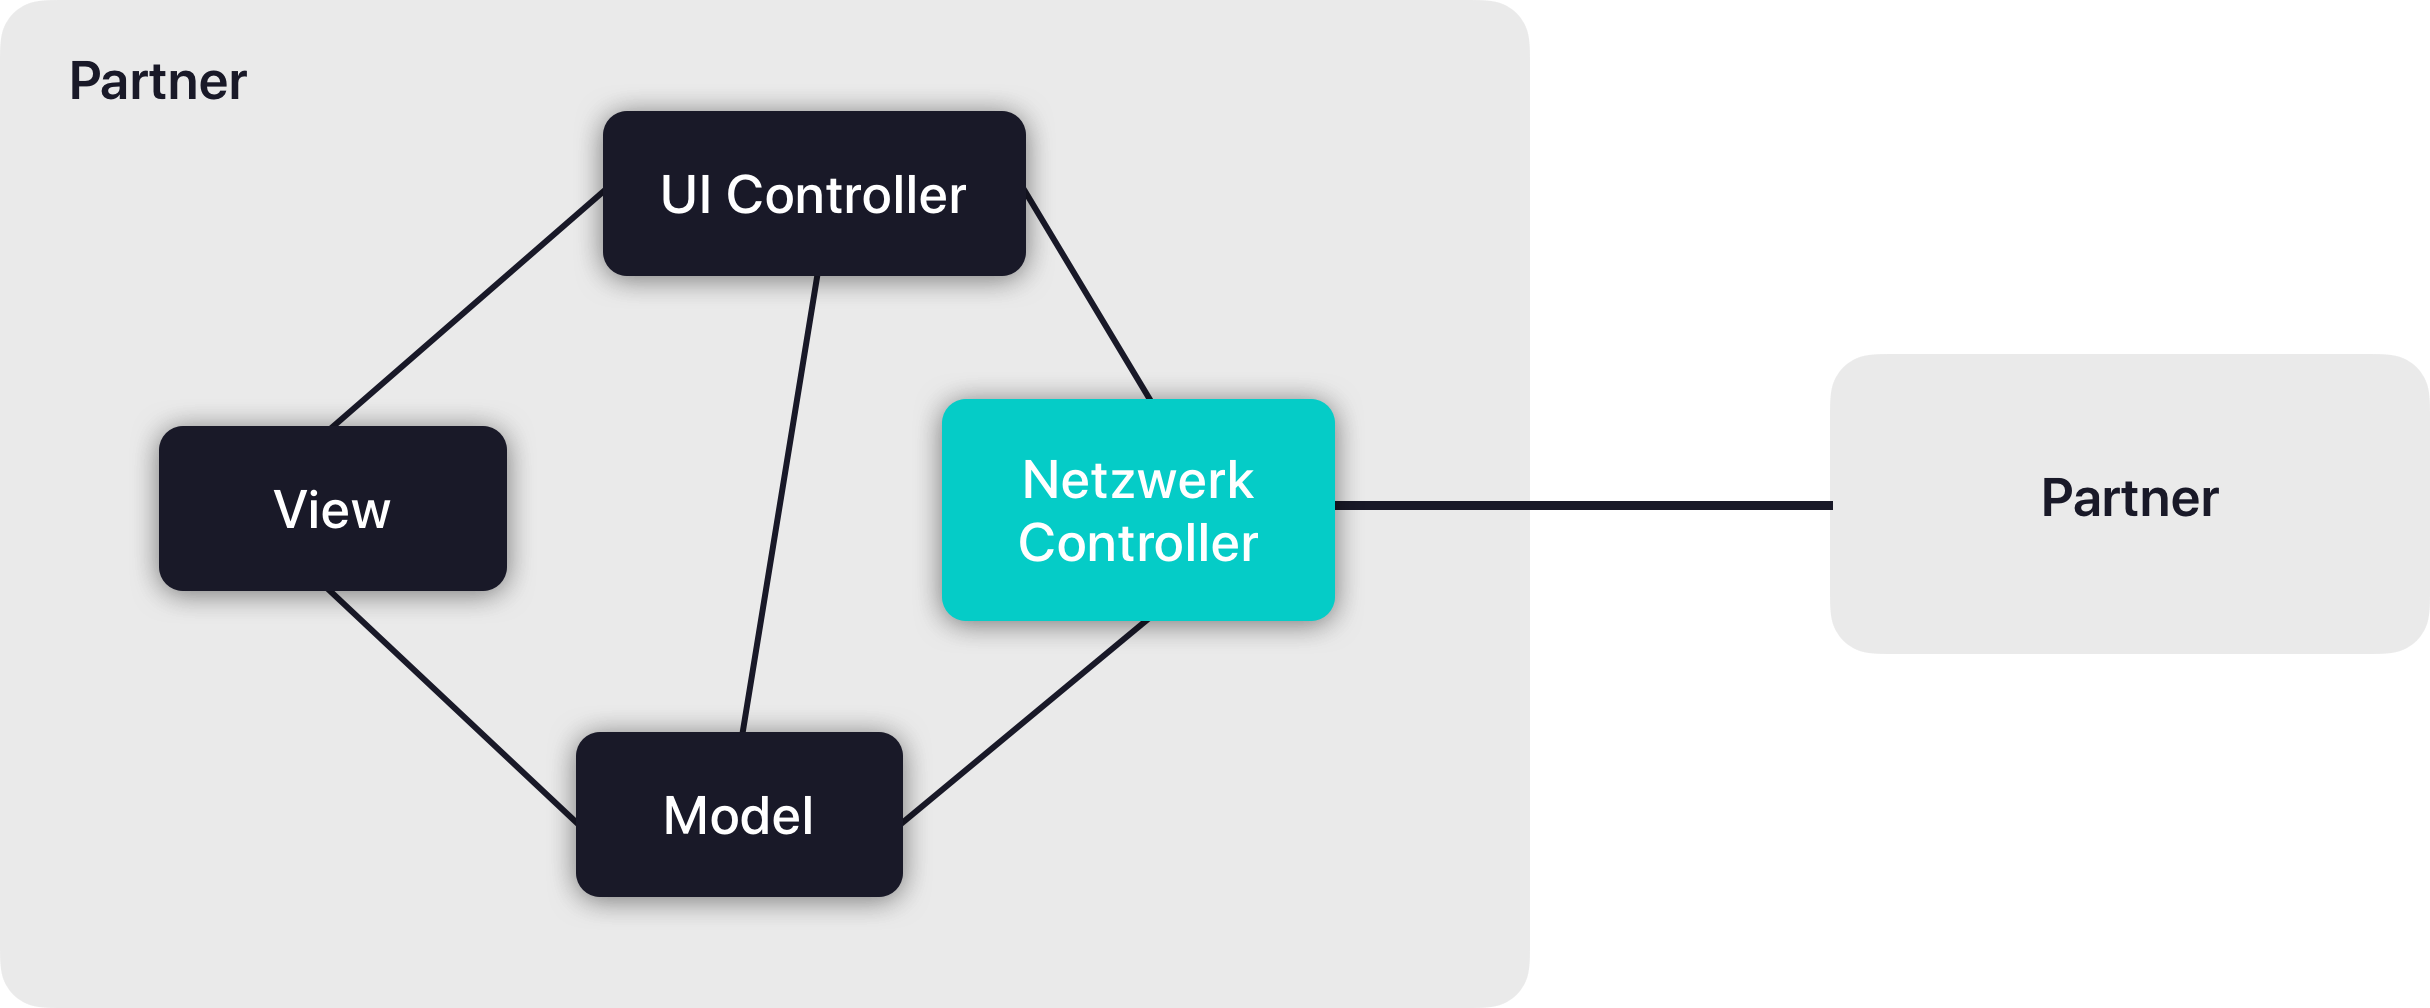
\includegraphics[width=1\textwidth]{graphics/Systemarchitektur}
  \caption{Schema der Systemarchitektur}
\end{figure}
Die Softwarearchitektur lässt sich auf zwei Ebenen betrachten, das Gesamtsystem mit Desktopanwendung des Arztes und mobilen Anwendung des Patienten und die Teilsysteme auf den jeweiligen Geräten. \\\\
Da die einzelnen Geräte im Gesamtsystem gleichberechtigt miteinander kommunizieren sollen, wird es als Partnernetz realisiert.\\\\
Die Teilsysteme auf den Nutzergeräten enthalten lokale Daten, die in einer graphischen Benutzeroberfläche dargestellt werden sollen. Um die Datenverwaltung von der Darstellung zu trennen, wird die Model-View-Controller Architektur verwendet.

\section{Szenarien}
\subsection{Szenario: Patient lädt sich neue Daten auf myMD}
Greg ist ein neuer Nutzer von myMD. Deshalb hat er auf seinem Konto auch noch keine Arztbriefe eingetragen. Also geht er zu seinem Hausarzt, um seine Krankenakte für die myMD \gls{App} zu erhalten. Der Arzt öffnet dafür seine Praxissoftware und exportiert alle Arztbriefe, die zu Greg gehören, und lädt diese in die \gls{Desktop Anwendung} von myMD. Sobald die Arztbriefe im Sendetool angezeigt werden, klickt der Arzt auf den Button "Daten senden". Nun erhält Greg in seiner myMD \gls{App} eine Meldung und klickt "Daten empfangen". Auf Gregs myMD \gls{App} erscheint jetzt die Nachricht, dass die Daten an ihn gesendet werden. Sobald der Sendeprozess beendet ist, kann der Arzt die \gls{Desktop Anwendung} von myMD schließen und sich dem nächsten Patienten widmen. Greg hat jetzt all seine Arztbriefe auf seinem Mobilgerät und kann sich diese jederzeit in der myMD \gls{App} anzeigen lassen. Sie werden im Tab "Übersicht" chronologisch sortiert dargestellt. Wenn er genauere Informationen zu einem bestimmten Arztbrief einsehen möchte, kann er auf den Arztbrief klicken und dieser wird nun auf dem ganzen Bildschirm, mit allen Informationen, dargestellt. So hat Greg jederzeit eine Übersicht

\subsection{Szenario: Eigene Daten ansehen und editieren}
Greg leidet seit einigen Tagen unter starken Magenbeschwerden. Sein Hausarzt findet keine Ursache für die Beschwerden und überweist ihn deshalb an den Spezialisten Dr. Haus und verschreibt ihm etwas gegen die Schmerzen. Dr. Haus glaubt die Ursache gefunden zu haben, diese lässt sich aber nur durch eine Operation beseitigen, für die er Greg an einen Chirurgen überweist. \\
Bevor er dem Eingriff zustimmt, will er sich noch eine zweite Meinung einholen. Dafür lässt er sich von seinem Hausarzt einen weiteren Spezialisten empfehlen, der jedoch keine medizinische Ursache für das Problem erkennen kann. Er empfiehlt Greg eine psychotherapeutische Behandlung und verschreibt ihm zur Überbrückung ein stärkeres Schmerzmittel. \\ 
Bei so vielen verschiedenen Ärzten und Diagnosen hat Greg nun etwas den Überblick verloren. Glücklicherweise hat er bei seinen Arztbesuchen myMD verwendet und hat nun alle relevanten Daten auf seinem Mobilgerät gesammelt und kann sich in der App einen Überblick verschaffen. Letztendlich entscheidet sich Greg, es mit der Psychotherapie zu versuchen und entfernt die nun überflüssigen, schwächeren Schmerzmittel aus der Liste seiner Medikationen in myMD. seiner Krankengeschichte.

\subsection{Szenario: Patient gibt behandelndem Arzt Daten zur Einsicht frei}
Gregs Beschwerden wollen kein Ende nehmen. Um der Ursache auf die Schliche zu kommen, überweist ihn sein Hausarzt nun an einen Gastroenterologen. Wie üblich bei neuen Patienten, möchte sich dieser zunächst mittels einer Anamnese einen Überblick über den Stand der Dinge verschaffen. Dank der myMD \gls{App} hat Greg jederzeit all seine Arztbriefe bei sich und kann diese nun seinem behandelnden Arzt zur Einsicht freigeben. Hierfür navigiert Greg in der myMD App in den Tab „Senden“, wo er nun aus einer Liste all seiner Arztbriefe jene auswählen kann, die er mit seinem Arzt teilen möchte. Greg entschließt sich dazu, nur Arztbriefe der letzten 6 Monate zu übertragen. \\
Per Knopfdruck beginnt das verschlüsselte Senden der Daten per \gls{Bluetooth} an den Computer des Arztes, auf welchem der Desktop-Klient von myMD die Daten verarbeitet und dem Arzt präsentiert. Schnell vermutet dieser, dass eine Wechselwirkung zwischen zwei eingenommenen Medikamenten die wahrscheinlichste Ursache für Gregs Leiden ist.

\section{Anwendungsfälle}
\subsection{Datenübertragung}
\begin{figure}[H]
\centering
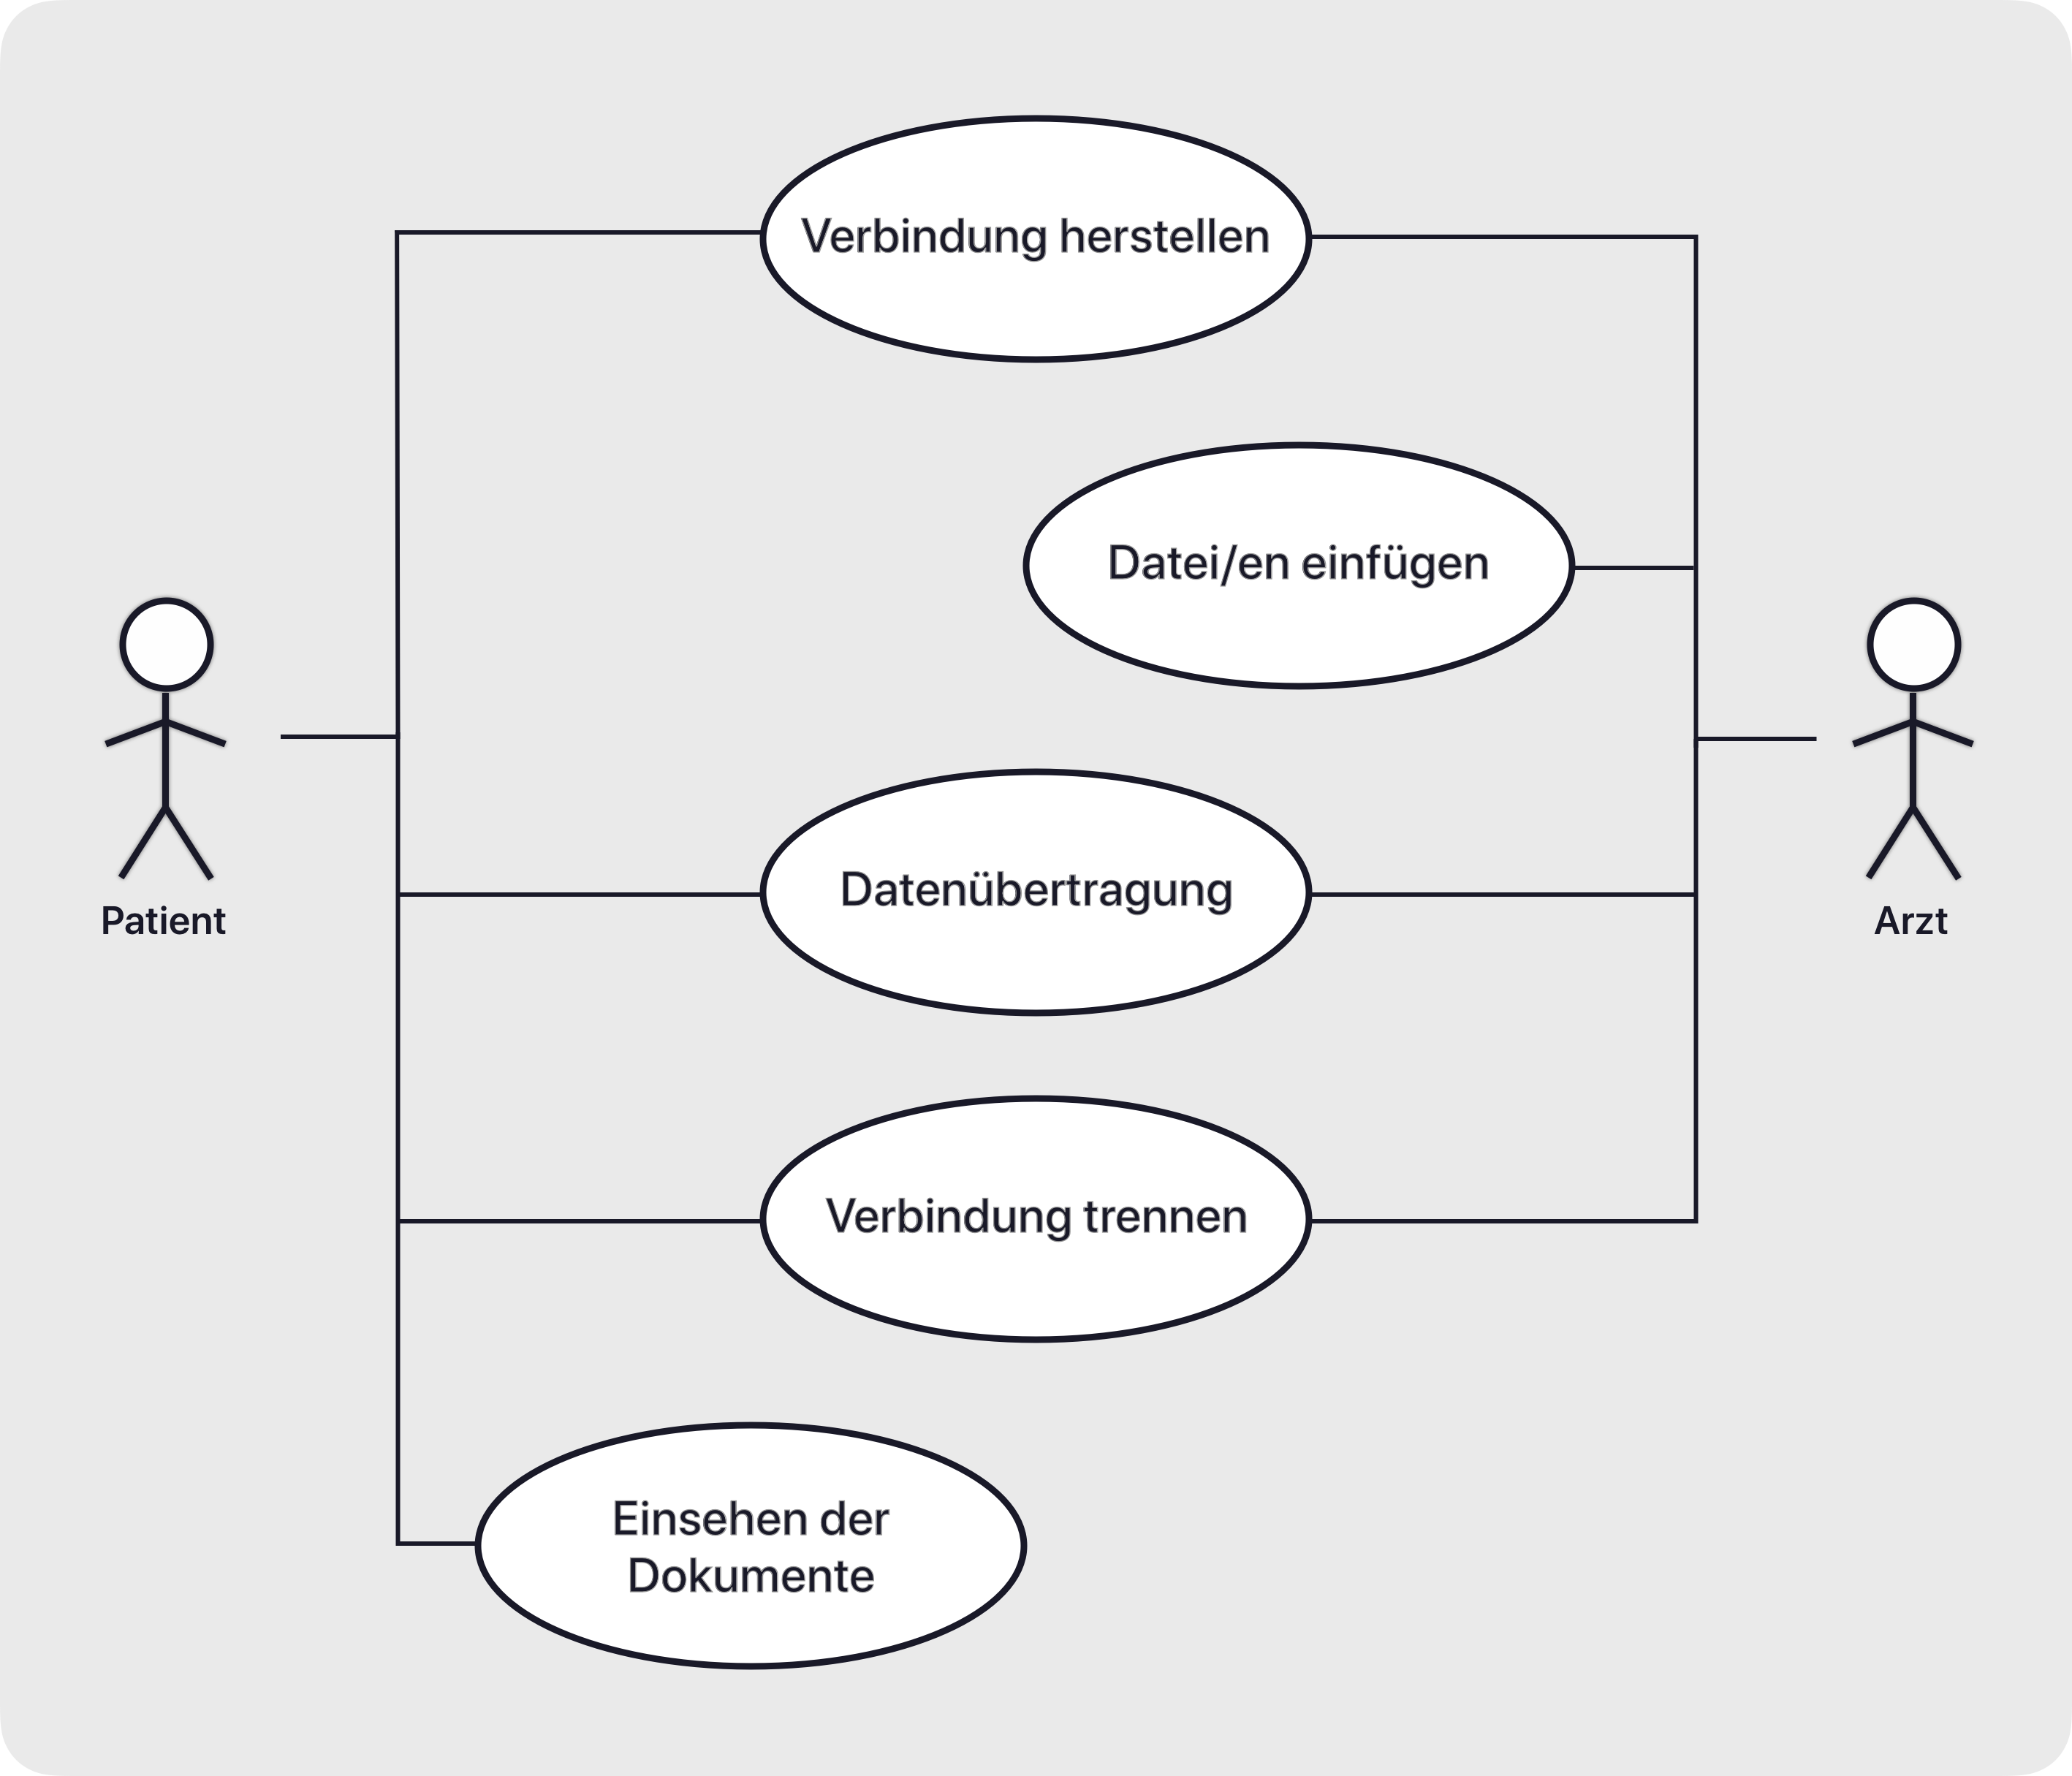
\includegraphics[width=0.8\textwidth]{graphics/AF-ArztPatient}
\caption{Anwendungsfall Datenübertragung Arzt-Patient}
\end{figure}

\begin{tabular}{lll}
{Name} & \multicolumn{2}{p{11.5cm}}  {Datenübertragung Arzt-Patient}\\
{Teilnehmende Akteure} & \multicolumn{2}{p{11.5cm}} {Patient, Arzt} \\
{Eingangsbedingung} & \multicolumn{2}{p{11.5cm}} {Der Patient hat die myMD \gls{App}, der Arzt die \gls{Desktop Anwendung} installiert} \\
{Ausgangsbedingung} & \multicolumn{2}{p{11.5cm}} {Die Daten wurden erfolgreich übertragen oder der Vorgang wird abgebrochen} \\
{Ereignisfluss} & \multicolumn{2}{p{11.5cm}} {Verbindung zwischen Arzt und Patienten wird hergestellt $\Rightarrow$ Arzt fügt zu übertragende Daten in die Anwendung ein $\Rightarrow$ Die Daten werden vom Arzt zum Patienten übertragen $\Rightarrow$ Verbindung zwischen Arzt und Patient wird getrennt $\Rightarrow$ Patient kann Daten einsehen} \\
{Spezielle Anforderungen} & \multicolumn{2}{p{11.5cm}} {Drahtlosverbindung zwischen Arzt und Patient} \\
\end{tabular} 

\subsection{Nutzerprofil}
\begin{figure}[H]
\centering
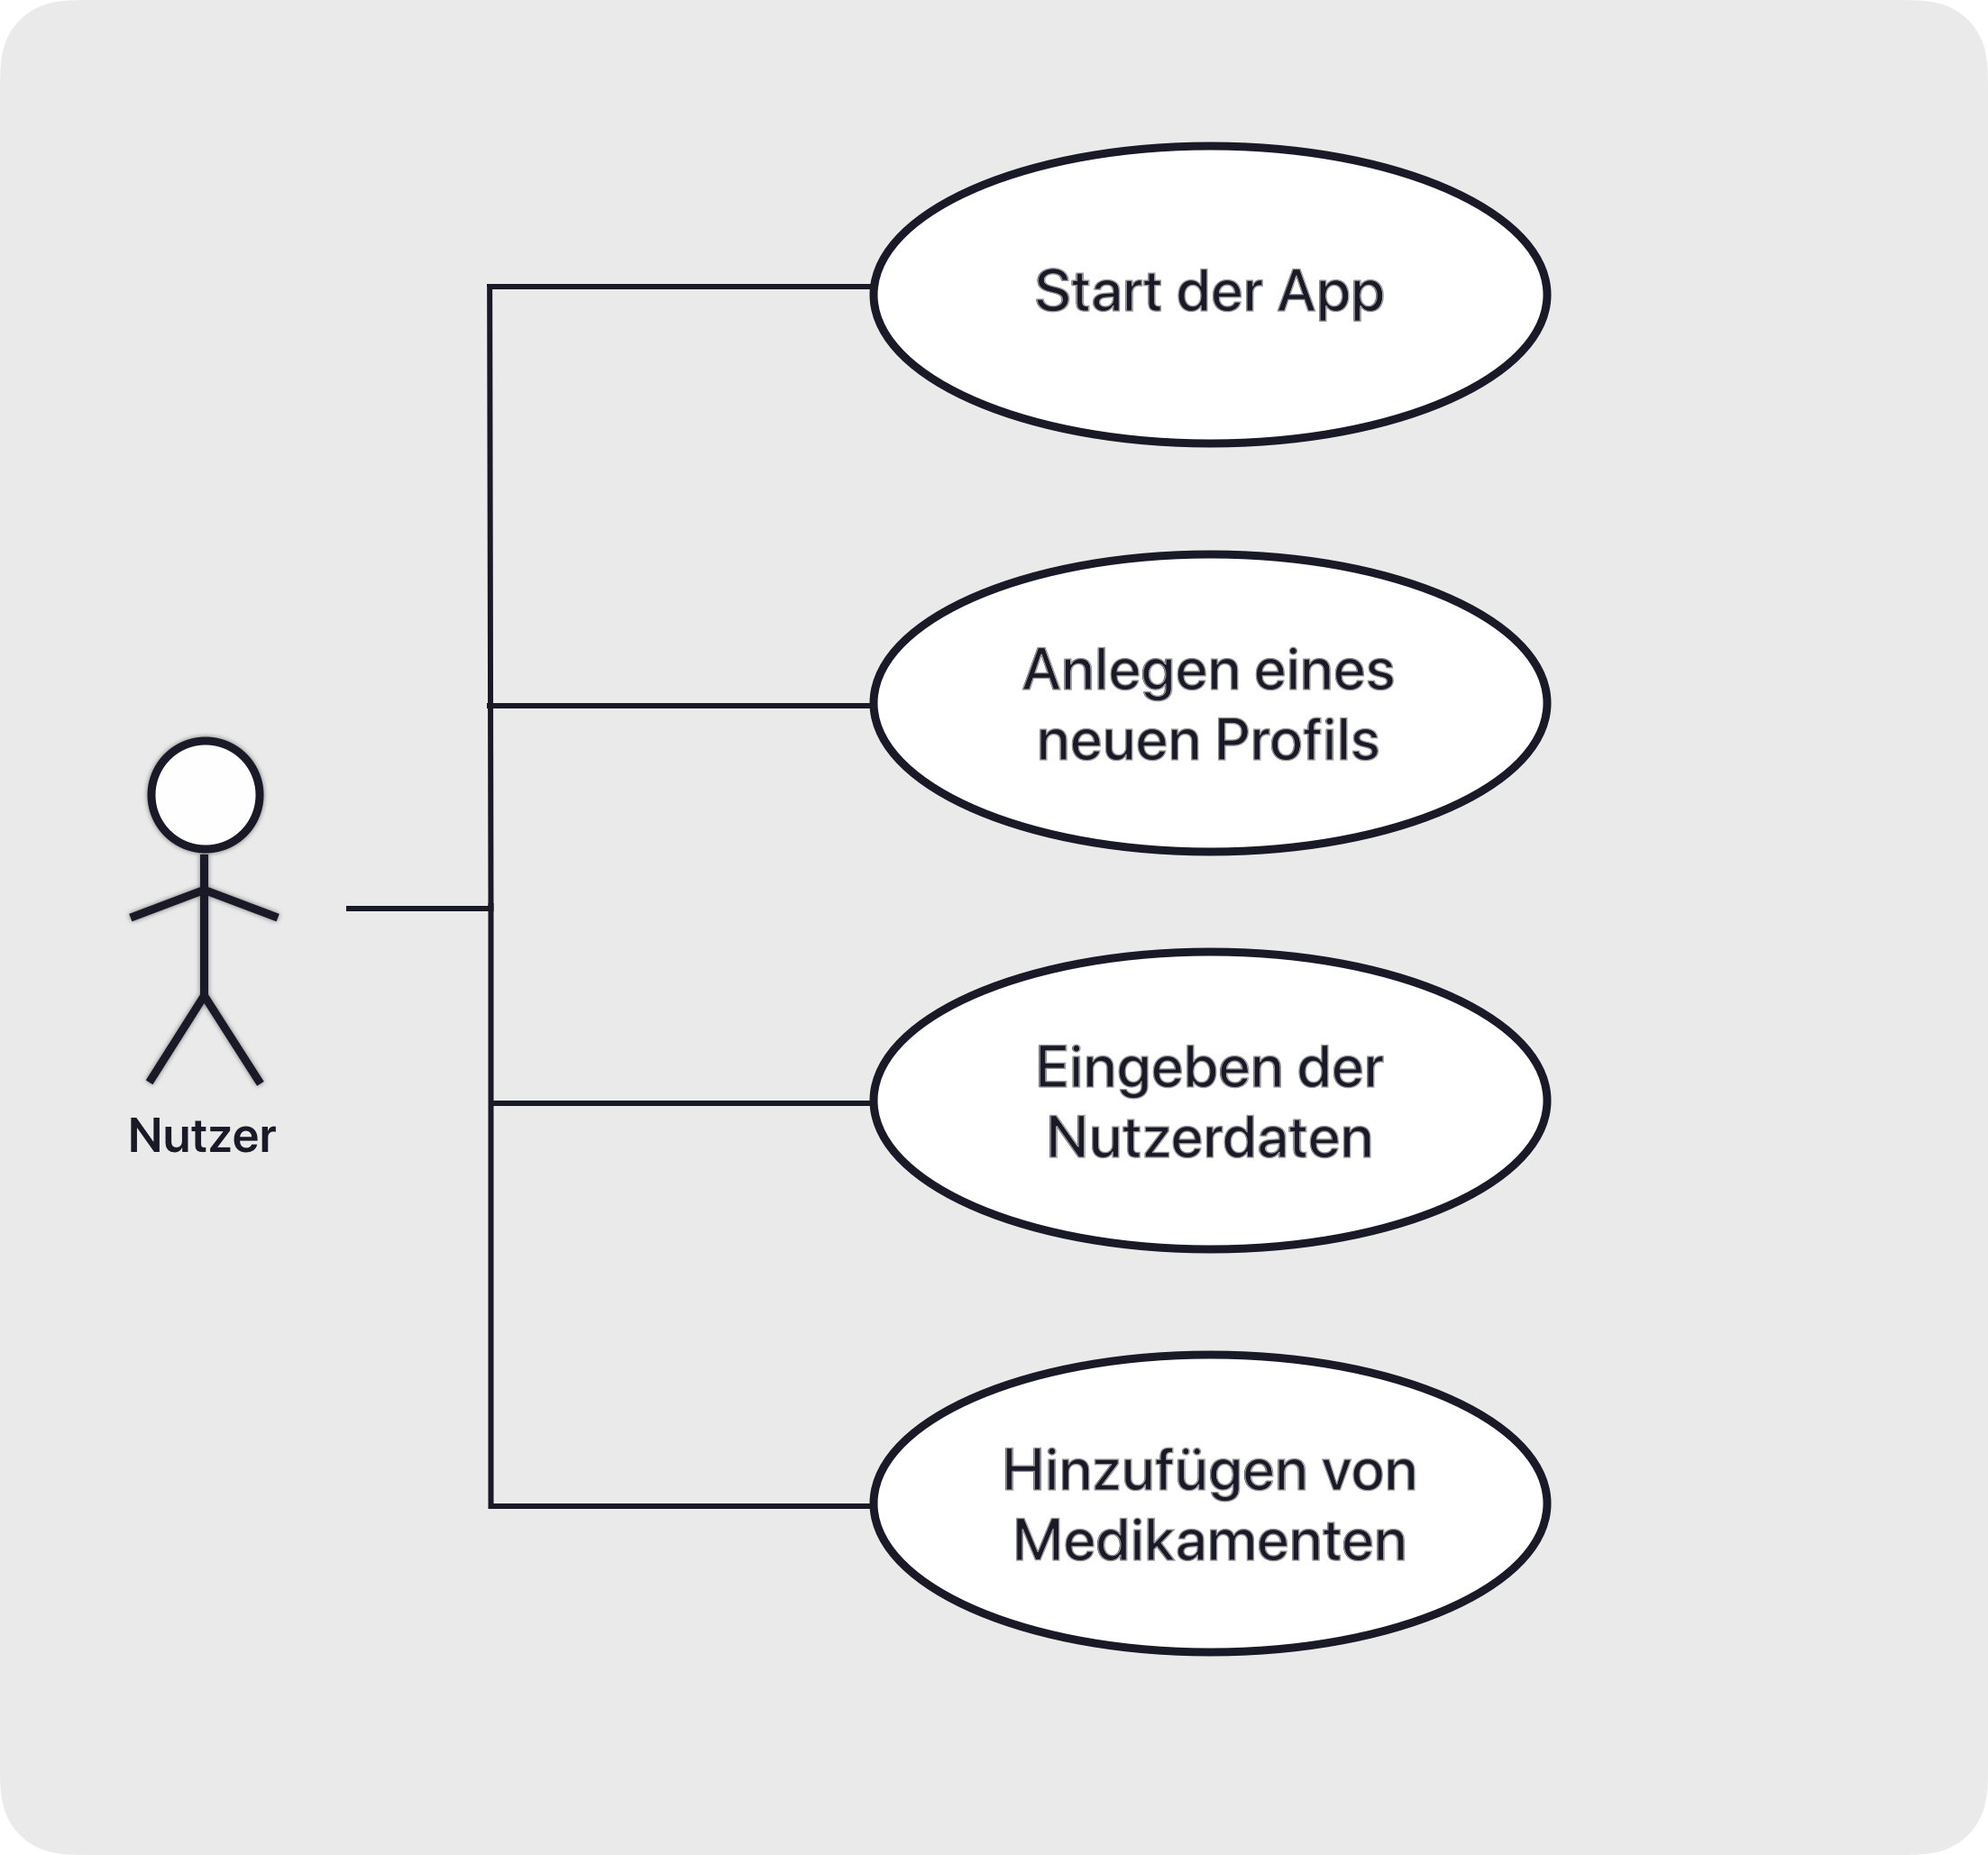
\includegraphics[width=0.8\textwidth]{graphics/AF-NeuerNutzer}
\caption{Anwendungsfall Neuer Nutzer}
\end{figure}

\begin{tabular}{lll}
{Name} & \multicolumn{2}{p{11.5cm}} {Neuer Nutzer}\\
{Teilnehmende Akteure} & \multicolumn{2}{p{11.5cm}} {Nutzer} \\
{Eingangsbedingung} & \multicolumn{2}{p{11.5cm}} {Der Nutzer hat die myMD \gls{App} installiert} \\
{Ausgangsbedingung} & \multicolumn{2}{p{11.5cm}} {Der Nutzer hat alle gewünschten Daten eingegeben oder den Vorgang abgebrochen} \\
{Ereignisfluss} & \multicolumn{2}{p{11.5cm}} {Ereignisfluss: Nutzer startet App $\Rightarrow$ Neues Profil erstellen $\Rightarrow$ Nutzer-Informationen eingeben $\Rightarrow$  Medikamente hinzufügen} \\
{Spezielle Anforderungen} & \multicolumn{2}{p{11.5cm}} {Keine} \\
\end{tabular} 

\section{Benutzungsoberfläche}
TODO: GUI Entwürfe  einbinden
\begin{figure}[ht]
  \centering
  \rule{8cm}{6cm}
  \caption{Dies könnte ein Bild der Benutzungsoberfläche sein}
\end{figure}

\chapter{Testfälle}
\section{Basis Testfälle (BT)}

\subsection{Patientenseitige Datenübertragung}
\begin{tabular}{lll}
[BT1010] & \multicolumn{2}{p{12cm}}  {\gls{Desktop Anwendung} sendet eine Datei an die myMD \gls{App}.} \\
{[BT1020]} & \multicolumn{2}{p{12cm}}  {Die Übertragung wird vom Nutzer unterbrochen.} \\
{[BT1030]} & \multicolumn{2}{p{12cm}}  {\gls{Desktop Anwendung} sendet ein unzulässige Datei (nicht unterstütztes Dateiformat).} \\
{[BT1040]} & \multicolumn{2}{p{12cm}}  {Die Übertragung wird durch äußere Umstände abgebrochen.} \\

\end{tabular}

\subsection{Darstellung}
\begin{tabular}{lll}
[BT2010] & \multicolumn{2}{p{12cm}}  {Ein neuer Arztbrief wird in eine leere Übersicht geladen.} \\
{[BT2020]} & \multicolumn{2}{p{12cm}}  {Ein neuer Arztbrief wird in bereits gefüllte Übersicht geladen.} \\
{[BT2030]} & \multicolumn{2}{p{12cm}}  {Ein digitaler Arztbrief wird angetippt/geöffnet.} \\
{[BT2040]} & \multicolumn{2}{p{12cm}}  {Ein digitaler Arztbrief wird geschlossen.} \\
{[BT2050]} & \multicolumn{2}{p{12cm}}  {Ein digitaler Arztbrief wird gelöscht.} \\

\end{tabular}

\subsection{Einstellungen}
\begin{tabular}{lll}
{[BT3010]} & \multicolumn{2}{p{12cm}}  {Das Nutzerprofil wird bearbeitet.} \\
\end{tabular}

\subsection{Desktop Anwendung}
\begin{tabular}{lll}
{[BT4010]} & \multicolumn{2}{p{12cm}}  {Unzulässige Datei wird zum Senden ausgewählt.} \\
{[BT4020]} & \multicolumn{2}{p{12cm}}  {Kompatible Datei wird zum Senden ausgewählt.} \\
{[BT4030]} & \multicolumn{2}{p{12cm}}  {Senden wird erfolgreich abgeschlossen.} \\
{[BT4040]} & \multicolumn{2}{p{12cm}}  {Senden wird durch äußere Einflüsse unterbrochen.} \\
{[BT4050]} & \multicolumn{2}{p{12cm}}  {Senden wird durch Nutzer unterbrochen.} \\
{[BT4060]} & \multicolumn{2}{p{12cm}}  {Geräte in der Nähe werden gesucht.} \\
{[BT4070]} & \multicolumn{2}{p{12cm}}  {Nutzergerät wird als Empfänger gewählt.} \\



\end{tabular}

\section{Erweiterte Testfälle (ET)}
\subsection{Patientenseitige Datenübertragung}
\begin{tabular}{lll}
[ET1010] & \multicolumn{2}{p{12cm}}  {myMD \gls{App} sendet eine Datei an die \gls{Desktop Anwendung}.} \\
{[ET1020]} & \multicolumn{2}{p{12cm}}  {myMD \gls{App} sendet mehrere Dateien an die \gls{Desktop Anwendung}.} \\
{[ET1030]} & \multicolumn{2}{p{12cm}}  {\gls{Desktop Anwendung} sendet mehrere Datei an die myMD \gls{App}.} \\
{[ET1040]} & \multicolumn{2}{p{12cm}}  {Die Übertragung mehrerer Daten wird durch äußere Umstände abgebrochen.} \\
{[ET1050]} & \multicolumn{2}{p{12cm}}  {Die Übertragung mehrerer Daten wird durch den Nutzer abgebrochen.} \\
{[ET1060]} & \multicolumn{2}{p{12cm}}  {Sensible Daten werden von der myMD App an die Desktop Anwendung gesendet.} \\
{[ET1070]} & \multicolumn{2}{p{12cm}}  {Die Verbindung wird über NFC hergetellt.} \\
{[ET1080]} & \multicolumn{2}{p{12cm}}  {Ein Profil wird auf ein anderes Gerät übertragen.} \\

\end{tabular}

\subsection{Darstellung}
\begin{tabular}{lll}
[ET2010] & \multicolumn{2}{p{12cm}}  {Medikament wird hinzugefügt.} \\
{[ET2020]} & \multicolumn{2}{p{12cm}}  {Medikament wird editiert.} \\
{[ET2030]} & \multicolumn{2}{p{12cm}}  {Medikament wird gelöscht.} \\
{[ET2040]} & \multicolumn{2}{p{12cm}}  {Laborwerte werden hinzugefügt.} \\
{[ET2050]} & \multicolumn{2}{p{12cm}}  {Laborwerte werden gelöscht.} \\{[ET2060]} & \multicolumn{2}{p{12cm}}  {Bilddatei wird hinzugefügt und dargestellt.} \\
{[ET2070]} & \multicolumn{2}{p{12cm}}  {Bilddatei wird mit einem Arztbrief verknüpft.} \\
{[ET2080]} & \multicolumn{2}{p{12cm}}  {Verknüpfung zwischen Arztbrief und Bilddatei wird getrennt.} \\
{[ET2090]} & \multicolumn{2}{p{12cm}}  {Überprüfung, ob eine Bilddatei originalgetreu ist.} \\
{[ET2100]} & \multicolumn{2}{p{12cm}}  {Mehrere Arztbriefe gruppieren.} \\
{[ET2110]} & \multicolumn{2}{p{12cm}}  {Einzelne Arztbriefe aus bestehender Gruppe entfernen.} \\
{[ET2120]} & \multicolumn{2}{p{12cm}}  {Nach eigen Gruppen sortieren.} \\
{[ET2130]} & \multicolumn{2}{p{12cm}}  {Überprüfen, ob Suchfunktion fehlerfrei funktioniert.} \\


\end{tabular}

\subsection{Einstellungen}
\begin{tabular}{lll}
[ET3010] & \multicolumn{2}{p{12cm}}  {Neues Nutzerprofil wird angelegt.} \\
{[ET3020]} & \multicolumn{2}{p{12cm}}  {Ein weiteres Nutzerprofil wird angelegt.} \\
{[ET3030]} & \multicolumn{2}{p{12cm}}  {Ein Nutzerprofil wird gelöscht.} \\
{[ET3040]} & \multicolumn{2}{p{12cm}}  {Wechsel zwischen mehreren Nutzerprofilen.} \\
{[ET3050]} & \multicolumn{2}{p{12cm}}  {Einzelnen Arztbrief als sensibel markieren.} \\
{[ET3060]} & \multicolumn{2}{p{12cm}}  {Sensibel Markierung eines einzelnen Arztbriefes aufheben.} \\
{[ET3070]} & \multicolumn{2}{p{12cm}}  {Gruppe von Arztbriefen als sensibel markieren.} \\
{[ET3080]} & \multicolumn{2}{p{12cm}}  {Sensibel Markierung einer Gruppe von Arztbriefen aufheben.} \\
{[ET3090]} & \multicolumn{2}{p{12cm}}  {Regelmäßiger Arzttermin wird hinzugefügt.} \\
{[ET3100]} & \multicolumn{2}{p{12cm}}  {Regelmäßiger Arzttermin wird gelöscht.} \\

\end{tabular}

\subsection{Desktop Anwendung}
\begin{tabular}{lll}
{[ET4010]} & \multicolumn{2}{p{12cm}}  {Datei mit falscher Versicherungsnummer wird gesendet.} \\


\end{tabular}

\section{Testszenarien (TS)}
\subsection{Typischer Arztbesuch}
Der Nutzer geht wegen einer Beschwerde zum Arzt und lässt sich untersuchen. Sobald die Untersuchung fertig ist, verlangt der Nutzer, dass der Arzt ihm die eben aufgenommenen Daten für die myMD \gls{App} zur Verfügung stellt. Der Arzt öffnet dann die \gls{Desktop Anwendung} und schickt dem Patienten den Arztbrief und Labordaten auf die myMD \gls{App}. Der Nutzer schaut sich dann kurz den neuen Eintrag in der Übersicht an, schließt die App und geht nach Hause. \newline

\begin{tabular}{lll}
[BT4060] & \multicolumn{2}{p{12cm}}  {Geräte in der Nähe werden gesucht.} \\
{[BT4070]} & \multicolumn{2}{p{12cm}}  {Das Mobilgerät des Nutzers wird als Empfänger ausgewählt.} \\
{[BT4030]} & \multicolumn{2}{p{12cm}}  {Senden wird erfolgreich abgeschlossen.} \\
{[BT2020]} & \multicolumn{2}{p{12cm}}  {Der neue Arztbrief wird in bereits gefüllte Übersicht geladen.} \\
{[ET2040]} & \multicolumn{2}{p{12cm}}  {Die Laborwerte werden hinzugefügt.} \\
{[BT2030]} & \multicolumn{2}{p{12cm}}  {Der neue Arztbrief wird geöffnet.} \\
{[BT2040]} & \multicolumn{2}{p{12cm}}  {Der neue Arztbrief wird geschlossen.} \\


\end{tabular}

\subsection{Krankenhistorie wird überprüft}
Der Nutzer ist daheim und schaut sich in der myMD \gls{App} seine Übersicht an. Er klickt auf einige Arztbriefe und liest sich durch, was darin steht. Dann bemerkt er, dass er alle Arztbriefe zu seinem gebrochenen Fuß gruppieren sollte und auch die Schmerzmittel, die für seinen Fuß bekommen hat, in den Tab Medikamente hinzufügen sollte. Versehentlich gibt er zuerst eine falsche Menge an, korrigiert diese aber und schließt daraufhin die App.\newline

\begin{tabular}{lll}
[BT2030] & \multicolumn{2}{p{12cm}}  {Ein Arztbrief wird geöffnet.} \\
{[BT2040]} & \multicolumn{2}{p{12cm}}  {Ein Arztbrief wird geschlossen.} \\
{[ET2100]} & \multicolumn{2}{p{12cm}}  {Alle Arztbriefe zum gebrochenen Fuß werden gruppiert.} \\
{[ET2010]} & \multicolumn{2}{p{12cm}}  {Medikament wird hinzugefügt.} \\
{[ET2020]} & \multicolumn{2}{p{12cm}}  {Medikament wird editiert.} \\

\end{tabular}

\subsection{Patient holt sich bei einem anderen Arzt eine zweite Meinung ein}
Der Nutzer hat eine sehr komplexe Beschwerde und will sich von einem anderen Arzt eine zweite Meinung einholen. Dazu geht er zu dem anderen Arzt und informiert ihn über die bisherige Diagnose, indem er ihm seine Arztbriefe von der myMD \gls{App} auf die \gls{Desktop Anwendung} schickt. Der Arzt schaut sich diese Arztbriefe in seiner Praxissoftware an, stellt seine eigene Diagnose, schreibt seinen Arztbrief und sendet ihn dem Patienten.\newline

\begin{tabular}{lll}
[ET1020] & \multicolumn{2}{p{12cm}}  {Die alten Arztbriefe werden dem Arzt gesendet.} \\
{[BT4060]} & \multicolumn{2}{p{12cm}}  {Geräte in der Nähe werden gesucht.} \\
{[BT4070]} & \multicolumn{2}{p{12cm}}  {Das Mobilgerät des Nutzers wird als Empfänger ausgewählt.} \\
{[BT4030]} & \multicolumn{2}{p{12cm}}  {Senden wird erfolgreich abgeschlossen.} \\

\end{tabular}

\subsection{Eine Mutter führt mehrere Profile}
Eine Mutter erstellt sich und ihrem Kind ein myMD Profil. Sie geht zum Arzt und lädt sich, zuerst für ihr eigenes Profil, alle Arztbriefe, die sie betreffen. Dann wechselt sie auf das Profil des Kindes und lädt sich wieder alle Arztbriefe in die App. Sobald das Kind seine eigene myMD App hat, überträgt die Mutter die alten Daten auf das Mobilgerät des Kindes. \newline

\begin{tabular}{lll}
[ET3010] & \multicolumn{2}{p{12cm}}  {Ein neues Nutzerprofil wird für die Mutter angelegt.} \\
{[ET3020]} & \multicolumn{2}{p{12cm}}  {Ein neues Nutzerprofil wird für das Kind angelegt.} \\
{[ET3030]} & \multicolumn{2}{p{12cm}}  {Es wird auf das Profil der Mutter gewechselt.} \\
{[ET1030]} & \multicolumn{2}{p{12cm}}  {Mehrere Dateien werden an die myMD App gesendet und auf das Profil der Mutter geladen.} \\
{[ET3030]} & \multicolumn{2}{p{12cm}}  {Es wird auf das Profil des Kindes gewechselt.} \\
{[ET1030]} & \multicolumn{2}{p{12cm}}  {Mehrere Dateien werden an die myMD App gesendet und auf das Profil der Mutter geladen.} \\
{[ET1080]} & \multicolumn{2}{p{12cm}}  {Das Profil des Kindes wird auf das Mobilgerät des Kindes übertragen.} \\

\end{tabular}



\chapter{Entwicklungsumgebung}
 
\section{Software}
\begin{tabular}{lll}
Entwicklungsumgebung &  \multicolumn{2}{p{12cm}}{Visual Studio 2017, Visual Studio for Mac}\\
Dokumentation &  \multicolumn{2}{p{12cm}}{Microsoft PowerPoint, LaTeX}  \\
GUI Entwürfe & \multicolumn{2}{p{12cm}}{Sketch} \\
Versionierung & \multicolumn{2}{p{12cm}}{Git, GitLab} \\
\end{tabular}

 
\section{Hardware}
\begin{tabular}{lll}
Omen by HP &  \multicolumn{2}{p{12cm}}{Intel Core i7-6700HQ CPU @ 2.60GHz \newline 16GB DDR3 RAM  \newline 64-Bit Microsoft Windows 10}\\
Custom Desktop PC &  \multicolumn{2}{p{12cm}}{Intel Xeon CPU E3-1231 v3 @ 3.40GHz \newline 8GB DDR3 RAM  \newline 64-Bit Microsoft Windows 10}\\
Apple MacBook Pro &  \multicolumn{2}{p{12cm}}{Intel Core i5-i5-2435M CPU @ 2.40GHz \newline 16GB DDR3 RAM  \newline Apple macOS 10.13}\\
\end{tabular}
 
 
\printnoidxglossaries

% Abbildungsverzeichnis
\listoffigures
 
\end{document}